% Options for packages loaded elsewhere
\PassOptionsToPackage{unicode}{hyperref}
\PassOptionsToPackage{hyphens}{url}
%
\documentclass[
  ignorenonframetext,
]{beamer}
\usepackage{pgfpages}
\setbeamertemplate{caption}[numbered]
\setbeamertemplate{caption label separator}{: }
\setbeamercolor{caption name}{fg=normal text.fg}
\beamertemplatenavigationsymbolsempty
% Prevent slide breaks in the middle of a paragraph
\widowpenalties 1 10000
\raggedbottom
\setbeamertemplate{part page}{
  \centering
  \begin{beamercolorbox}[sep=16pt,center]{part title}
    \usebeamerfont{part title}\insertpart\par
  \end{beamercolorbox}
}
\setbeamertemplate{section page}{
  \centering
  \begin{beamercolorbox}[sep=12pt,center]{part title}
    \usebeamerfont{section title}\insertsection\par
  \end{beamercolorbox}
}
\setbeamertemplate{subsection page}{
  \centering
  \begin{beamercolorbox}[sep=8pt,center]{part title}
    \usebeamerfont{subsection title}\insertsubsection\par
  \end{beamercolorbox}
}
\AtBeginPart{
  \frame{\partpage}
}
\AtBeginSection{
  \ifbibliography
  \else
    \frame{\sectionpage}
  \fi
}
\AtBeginSubsection{
  \frame{\subsectionpage}
}

\usepackage{amsmath,amssymb}
\usepackage{iftex}
\ifPDFTeX
  \usepackage[T1]{fontenc}
  \usepackage[utf8]{inputenc}
  \usepackage{textcomp} % provide euro and other symbols
\else % if luatex or xetex
  \usepackage{unicode-math}
  \defaultfontfeatures{Scale=MatchLowercase}
  \defaultfontfeatures[\rmfamily]{Ligatures=TeX,Scale=1}
\fi
\usepackage{lmodern}
\ifPDFTeX\else  
    % xetex/luatex font selection
\fi
% Use upquote if available, for straight quotes in verbatim environments
\IfFileExists{upquote.sty}{\usepackage{upquote}}{}
\IfFileExists{microtype.sty}{% use microtype if available
  \usepackage[]{microtype}
  \UseMicrotypeSet[protrusion]{basicmath} % disable protrusion for tt fonts
}{}
\makeatletter
\@ifundefined{KOMAClassName}{% if non-KOMA class
  \IfFileExists{parskip.sty}{%
    \usepackage{parskip}
  }{% else
    \setlength{\parindent}{0pt}
    \setlength{\parskip}{6pt plus 2pt minus 1pt}}
}{% if KOMA class
  \KOMAoptions{parskip=half}}
\makeatother
\usepackage{xcolor}
\newif\ifbibliography
\setlength{\emergencystretch}{3em} % prevent overfull lines
\setcounter{secnumdepth}{-\maxdimen} % remove section numbering


\providecommand{\tightlist}{%
  \setlength{\itemsep}{0pt}\setlength{\parskip}{0pt}}\usepackage{longtable,booktabs,array}
\usepackage{calc} % for calculating minipage widths
\usepackage{caption}
% Make caption package work with longtable
\makeatletter
\def\fnum@table{\tablename~\thetable}
\makeatother
\usepackage{graphicx}
\makeatletter
\def\maxwidth{\ifdim\Gin@nat@width>\linewidth\linewidth\else\Gin@nat@width\fi}
\def\maxheight{\ifdim\Gin@nat@height>\textheight\textheight\else\Gin@nat@height\fi}
\makeatother
% Scale images if necessary, so that they will not overflow the page
% margins by default, and it is still possible to overwrite the defaults
% using explicit options in \includegraphics[width, height, ...]{}
\setkeys{Gin}{width=\maxwidth,height=\maxheight,keepaspectratio}
% Set default figure placement to htbp
\makeatletter
\def\fps@figure{htbp}
\makeatother

\makeatletter
\@ifpackageloaded{caption}{}{\usepackage{caption}}
\AtBeginDocument{%
\ifdefined\contentsname
  \renewcommand*\contentsname{Table of contents}
\else
  \newcommand\contentsname{Table of contents}
\fi
\ifdefined\listfigurename
  \renewcommand*\listfigurename{List of Figures}
\else
  \newcommand\listfigurename{List of Figures}
\fi
\ifdefined\listtablename
  \renewcommand*\listtablename{List of Tables}
\else
  \newcommand\listtablename{List of Tables}
\fi
\ifdefined\figurename
  \renewcommand*\figurename{Figure}
\else
  \newcommand\figurename{Figure}
\fi
\ifdefined\tablename
  \renewcommand*\tablename{Table}
\else
  \newcommand\tablename{Table}
\fi
}
\@ifpackageloaded{float}{}{\usepackage{float}}
\floatstyle{ruled}
\@ifundefined{c@chapter}{\newfloat{codelisting}{h}{lop}}{\newfloat{codelisting}{h}{lop}[chapter]}
\floatname{codelisting}{Listing}
\newcommand*\listoflistings{\listof{codelisting}{List of Listings}}
\makeatother
\makeatletter
\makeatother
\makeatletter
\@ifpackageloaded{caption}{}{\usepackage{caption}}
\@ifpackageloaded{subcaption}{}{\usepackage{subcaption}}
\makeatother
\ifLuaTeX
  \usepackage{selnolig}  % disable illegal ligatures
\fi
\usepackage{bookmark}

\IfFileExists{xurl.sty}{\usepackage{xurl}}{} % add URL line breaks if available
\urlstyle{same} % disable monospaced font for URLs
\hypersetup{
  pdftitle={Financial Intermediation},
  pdfauthor={Pablo Winant},
  hidelinks,
  pdfcreator={LaTeX via pandoc}}

\title{Financial Intermediation}
\subtitle{Macro II - Fluctuations - ENSAE, 2023-2024}
\author{Pablo Winant}
\date{2024-04-10}

\begin{document}
\frame{\titlepage}

\begin{frame}{The Model}
\phantomsection\label{the-model}
discrete-time economy. The economy features three agents: households,
bankers, and entrepreneurs.

\begin{block}{Summary}
\phantomsection\label{summary}
I consider a discrete-time economy. The economy features three agents:
households, bankers, and entrepreneurs. Each agent has a unit mass.4
Households work, consume and buy real estate, and make one-period
deposits into a bank. The household sector in the aggregate is net
saver. Entrepreneurs accumulate real estate, hire households, and borrow
from banks. In between the households and the entrepreneurs, bankers
intermediate funds. The nature of the banking activity implies that
bankers are borrowers when it comes to their relationship with
households, and are lenders when it comes to their relationship with the
credit-dependent sector -- the entrepreneurs. I design preferences in a
way that two frictions coexist and interact in the model's equilibrium:
first, bankers are credit constrained in how much they can borrow from
the patient savers; second, entrepreneurs are credit constrained in how
much they can borrow from bankers.
\end{block}

\begin{block}{Households}
\phantomsection\label{households}
Representative agent chooses housing \(H_{H,t}\), consumption
\(C_{T,t}\) and time spent working \(N_{H,t}\) to solve

\[\max E_t \sum_{t=0}^{\infty} \beta^t_H \left( \log C_{H,t} + j \log H_{H,t} + \tau \log(1-N_{H,t}) \right)\]

where \(\beta_{H,t}\) is the discount factor

\pause

Budget constraint:

\(C_{H,t} + D_t + q_t \left( H_{H,t}- H_{H,t-1} \right) = R_{H,t-1} D_{t-1} + W_{H,t} N_{H,t} + \epsilon_t\)

where:

\begin{itemize}
\tightlist
\item
  \(D_t\): bank deposits earning gross return \(R_{H,t}\)
\item
  \(q_t\): price of housing
\item
  \(W_t\): wage rate
\item
  \(\epsilon_t\): is a redistributive shock
\end{itemize}
\end{block}

\begin{block}{Households: Optimality conditions}
\phantomsection\label{households-optimality-conditions}
\[\frac{1}{C_{H,t}} = \beta_H E_t \left( \frac{1}{C_{H,t+1}} R_{H,t} \right)\]
\[\frac{q_t}{C_{H,t}} = \frac{j}{H_{H,t}} + \beta_H E_t \left( \frac{q_{t+1}}{C_{H,t+1}}  \right)\]
\[\frac{W_{H,t}}{C_{H,t}} = \frac{\tau}{1-N_{H,t}}\]
\end{block}

\begin{block}{Entrepreneurs}
\phantomsection\label{entrepreneurs}
The representative entrepreneur chooses consumption \(C_{E,t}\), housing
\(H_{H,t}\), produces \(Y_t\) by remunerating \(N_{H,t}\) hours from
workers.

\[\max E_0 \sum_{t=0}^{\infty} \beta^t_E \log C_{E,t}\]

subject to:

\[C_{E,t} + q_t \left( H_{E,t} - H_{E,t-1} \right) + R_{E,t} L_{E,t-1} + W_{H,t} N_{H,t} + a c_{EE,t} = Y_t + L_{E,t}\]

\[Y_t = H^{\nu}_{E,t-1} N^{1-\nu}_{H,t}\]

\begin{equation}\phantomsection\label{eq-borrowing-constraint}{
L_{E,t} \leq m_H E_t \left( \frac{q_{t+1}}{R_{E,t+1}}H_{E,t} \right) - m_N W_{H,t} N_{H,t}
}\end{equation}

\begin{itemize}
\item
  \(L_{E,t}\) are loans to the entrepreneur with gross return
  \(R_{E,t}\)
\item
  \(c_{EE,t}=\frac{\phi_{EE}}{2}\frac{\left(L_{E,t}-L_{E,t-1}\right)}{L_E}\)
  with \(L_E\) the steady-state of \(L_{E,t}\) \footnote<.->{the
    quadratic adjustment cost is assumed to be \emph{external} to the
    banker}

  \begin{itemize}
  \tightlist
  \item
    captures the fact that loans change slowly
  \end{itemize}
\end{itemize}

Equation~\ref{eq-borrowing-constraint}: borrowing constraint

\begin{itemize}
\tightlist
\item
  entrepreneurs cannot borrow more than a fraction \(m_H\) of the
  expected value of their real estate stock
\item
  a fraction \(m_N\) of the wage bill must be paid in advance
\end{itemize}

Assumption: entrepreneurs discount future more than housholds and
bankers

\[\beta_E < \frac{1}{\gamma_E \frac{1}{\beta_H} + (1-\gamma_E)\frac{1}{\beta_B}}\]
with \(\gamma_E\in[0,1]\)\$

\textbf{Remarks?}
\end{block}

\begin{block}{Intepretation on the lagrange multiplier?//}
\phantomsection\label{intepretation-on-the-lagrange-multiplier}
\end{block}

\begin{block}{Bankers}
\phantomsection\label{bankers}
The representative banker maximizes private consumption \(C_{B,t}\)

\[\max E_0 \sum_{t=0}^{\infty} \beta^t_B \log C_{B,t}\]

subject to:

\[C_{B,t} + R_{H,t-1} D_{t-1} + L_{E,t} + a c_{EB,t} = D_t + R_{E,t} L_{E,t-1} - \epsilon_t\]

where:

\begin{itemize}
\item
  \(D_t\): households deposits
\item
  \(L_{E,t}\): loans to entrepreneurs
\item
  \(a c_{EB,t} = \frac{\phi_{EB}}{2} \frac{(L_{E,t-L_{E,t-1}})^2}{L_E}\)
  is quadratic adjustment cost\footnote<.->{the quadratic adjustment
    cost is assumed to be \emph{external} to the banker}
\item
  the ability convert deposits into loans is limited by a capital to
  assets ratio yielding a borrowing constraint\footnote<.->{here capital
    ratio is
    \(D_t \leq \gamma_E \left( L_{E,t} - E_t \epsilon_{t+1} \right)\)}
\end{itemize}

\[D_t \leq \gamma_E \left( L_{E,t} - E_t \epsilon_{t+1} \right)\]
\end{block}

\begin{block}{Bankers (optimality)}
\phantomsection\label{bankers-optimality}
Denote:

\begin{itemize}
\tightlist
\item
  \(m_{B,t} = \beta_B E_t \left( \frac{C_{B,t}}{C_{B,t+1}}\right)\): the
  stochastic discount factor of the banker
\item
  \(\lambda_{B,t}\): multiplier on the capital adequacy constraint
  \emph{normalized by marginal utiliy of consumption}
\end{itemize}

Optimality conditions:

\begin{equation}\phantomsection\label{eq-foc-banker-1}{1-\lambda_{B,t} = E_t \left( m_{B,t} R_{H,t} \right)}\end{equation}

\begin{equation}\phantomsection\label{eq-foc-banker-2}{1-\gamma_{E} \lambda_{B,t} + \frac{\partial ac_{EB,t}}{\partial L_{E,t}} = E_t \left( m_{B,t} R_{E,t+1} \right)}\end{equation}

These two equations explain the spread between the deposit rate and the
lending rate (aka the intermediation premium)
\end{block}

\begin{block}{Bankers (temp)}
\phantomsection\label{bankers-temp}
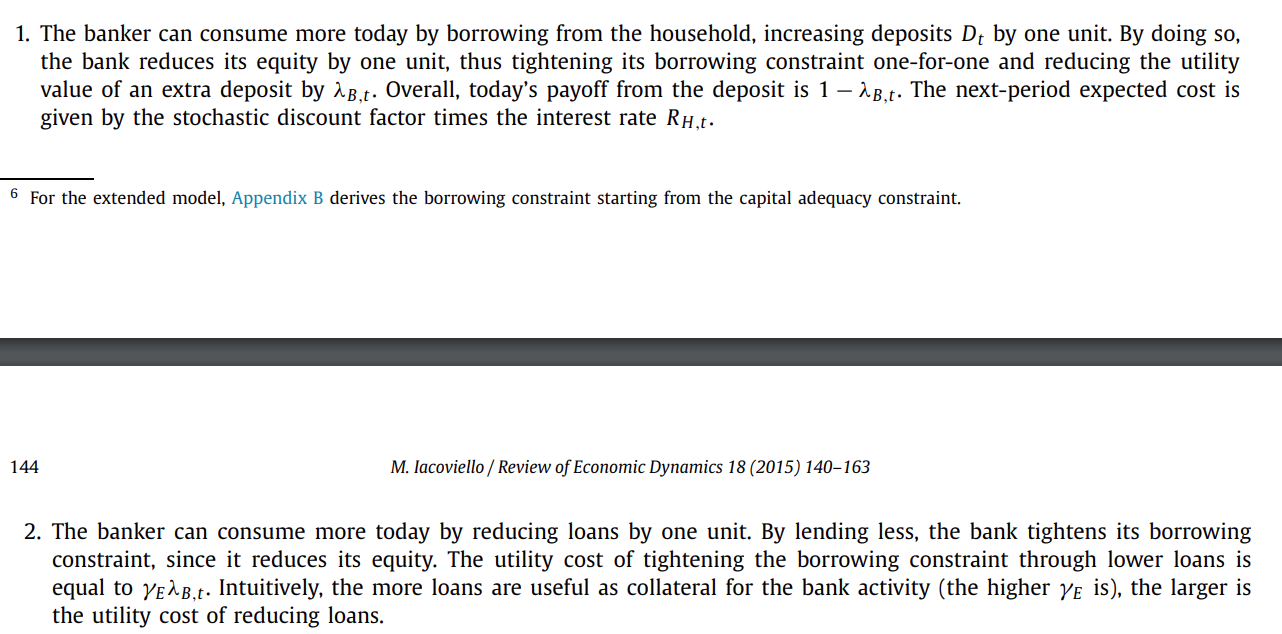
\includegraphics{assets/explanations.png}
\end{block}

\begin{block}{Market clearing}
\phantomsection\label{market-clearing}
Total supply of housing \(H_{E,t} + H_{H,t} = 1\)

Market clearing conditions for goods and housing:

\[H_{E,t} + H_{H,t} = 1\]
\end{block}

\begin{block}{Steady state properties}
\phantomsection\label{steady-state-properties}
For the household:

\[R_H=\frac{1}{\beta_H}\]

For the banker:

Equation~\ref{eq-foc-banker-1} and Equation~\ref{eq-foc-banker-2} imply
that as long as \(\beta_B<\beta_H\), the bankers are credit constrained

With \(\gamma_{E}\) smaller than one, there is a spread between return
on loans and return on deposits:

\[\lambda_B = 1-\beta_B R_H = 1-\frac{\beta_B}{\beta_H}>0\]

\[R_E = \frac{1}{\beta_B} - \gamma_E \left( \frac{1}{\beta_B} - \frac{1}{\beta_H} \right)>R_H\]

For entrepreneurs

Entrepreneurs are constrained if \(\beta_E R_E<1\). that is equivalent
to
\[\frac{1}{\beta_E}=\gamma_E \frac{1}{\beta_H} + (1-\gamma_E) \frac{1}{\beta_B}\]

Effect:

\begin{itemize}
\tightlist
\item
  banker's credit constraint and entrepreneur credit constraint create a
  wedge amd reduce steady-state output
\end{itemize}
\end{block}

\begin{block}{Calibration}
\phantomsection\label{calibration}
Time period: 1 quarter

Time discounts: - households: \(\beta_H=0.9925\) - bankers:
\(\beta_B=0.945\) - entrepreneurs: \(\beta_E=0.94\)

Choice of leverage parameters such that \(R_H=3%
\) and \(R_E=5%
\).

Adjustment costs: \(\phi_{EE}=\phi_{EB}=0.25\)

Wieght of leisure: \(\tau=2\) (active time spent=1/2 and Frisch
elasticity close to 1).

Share of housing in production: \(\nu=0.05\)

Preference parameter for housing \(j=0.075\): ration of real estate
wealth to output 3.1 (0.8 commercial, 2.3 residential)

Leverage: - \(m_N=1\): all labour paid in advance - \(m_H=0.9\):
entrepreneur loan-to-value (LTV) - \(\gamma_E=0.9\): bank leverage
(close to historical capital asset ratios close to 1)
\end{block}

\begin{block}{Dynamics}
\phantomsection\label{dynamics}
Intuition

\[E_t \left( R_{E,t+1} \right) - R_H,t = \frac{\lambda_{B,t}}{m_{B,t}}(1-\gamma_E)\]

\begin{itemize}
\tightlist
\item
  price side:
\end{itemize}

When the multiplier on the banker's constraint becomes larger the spread
increases

\begin{itemize}
\tightlist
\item
  quantity side:
\end{itemize}
\end{block}

\begin{block}{Simulation}
\phantomsection\label{simulation}
Shock \(\epsilon_t\) calibrated on historical loan losses.

\[Follows $\epsilon_t = 0.9 \epsilon_{t-1} + \iota_t\]

\ldots details about the shock
\end{block}
\end{frame}



\end{document}
